\chapter{Struktur}
\section{Basics}
Da vi skulle planlægge projektet valgte vi efter en brainstorm at dele projektet op i en mængde delmål vi ville have implementeret. Delmålene i kategorien basics var dem vi skulle implementere for at have et fungerende spil. Vi fandt frem til at det ville være følgende funktionaliteter:
\begin{itemize}
\item \textbf{Keyboard input}
\item \textbf{Bevægelig bold og striker (med clear)}
\item \textbf{Reflex-logik på kanter og hjørner}
\item \textbf{Game start og game over}
\end{itemize}
Vi vil i det følgende forklare hvordan disse delmål blev implementeret. 

Hvordan implementerede vi keyboardinput?
\texttt{kode tekst tekst}

\subsection{Keyboard input}


\section{Advanced}
Efter alle basics var færdigimplementeret, havde vi planlagt at lave nogle mindre udvidelser til spillet. Disse omfatter dels implemention af liv og pointsystem, men også videreudviklinger af basic-funktionaliteterne, sådan så deres bagvedliggende virkemåde gøres mere avanceret. Advanced inkulderer følgende.

\begin{itemize}
\item \textbf{Liv}. Som i ethvert andet arkade-spil har vi implementeret liv, sådan så man starter med tre og bliver Game Over, når der er nul liv tilbage.

\item \textbf{Score}. Point-systemet er opbygget sådan så det giver 1 point hver gang man rammer en brik og et ekstra point når brikken dør (går fra 1 til 0 liv). Det giver ingen point når bolden rammer strikeren, hvilket skyldes at man ikke skal have credit for tålmodighed.

\item \textbf{Hastighed}. Hastigheden hvormed bolden bevæger sig afhænger dels af hvor mange point man har, dels af hvilken sværhedsgrad man spiller på. På easy bliver boldens hastighed sat op for hver 10. point man får, på medium for hver 5. point man får, på hard for hver 2. point man får og på Chuck Norris, tja hvem ved?

\item \textbf{Vilkårlig startvinkel}. Når bolden skydes af bliver den sendt afsted i en vilkårlig vinkel på mellem 45 og 135 grader. Det vil sige lodret op fra strikeren plus minus op til 45 grader. Dette er implementeret for at man ikke kan time startvinklen så man er sikker på den altid rammer et bestemt sted.

\item \textbf{Striker-zoner}. Strikeren er opbygget sådan så den altid skal bestå af et lige antal felter. Dens midterste venstre felt har en afbøjningsvinkel på indgangsvinkel plus 0 grader, og dens yderste venstre felt har en afbøjningsvinkel på indgangsvinkel plus 45 grader. Hvert felt mellem det midterste venstre til det yderste venstre felt, har så en stigende afbøjningsvinkel, hvor den vinkel der bliver lagt til hvert felt er 45 grader divideret med antallet af felter fra det midterstre venstre (eksklusiv) til det yderstre venstre (eksklusiv). Højre-siden af strikeren fungerer på præcis samme måde, bare med omvendt fortegn, sådan så afbøjningsvinklen på midterste højre felt er lig indgangsvinklen og afbøjningsvinklen på yderstre højre felt er lig indgangsvinklen minus 45 grader.\\

Strikeren er lavet på denne måde så dens bredde er meget fleksibel. Fx bruges der forskellige Striker-størrelser på spillets forskellige sværhedsgrader og dette er så bare implementeret ved at ændre på størrelsen af \texttt{striker.width}. Så sørger spillet selv for at inddele Striker-zonerne. 

\item \textbf{Internt 18.14 koordinat-system}. I basic-implementationen af spillet satte vi bolden til at rykke sig et bestem antal monospaces hver gang den bevægede sig. Men med denne implementation er hele banens indre struktur blevet gentænkt sådan så bolden bevæger sig som en vektor i et koordinatsystem. Vi har lavet en \texttt{Ball struct} sådan så bolden hele tiden kender sine egne (x,y)-koordinater, samt dens egen enhedsvektor (altså retning hvori den bevæger sig). Når bolden bevæger sig sker der det at dens vektors (x,y)-koordinat lægges til boldens (x,y)-koordinat. Derefter tjekkes om bolden er død eller har ramt en brik, en væg, et hjørne, strikeren eller loftet. Hvis intet af dette er tilfældet, slettes boldens gamle koordinater ved at der på disse felter tegnes blanke mellemrum. Derefter afrundes boldens (x,y)-koordinater til nærmeste heltal ved at kigge på 1. bit efter kommaet, det vil sige boldens x- hhv. y-koordinats 19. bit (Da det tænkte komma er sat mellem 18. og 19. bit). Hvis denne er 0 rundes ned og ellers rundes op. Nu kendes boldens (x,y)-koordinat i heltal og den kan derfor indtegnes på banen.\\


\item \textbf{bolden bevæger sig med samme hastighed i både x- og y-retning}. Vi havde et problem med at det på skærmen lignede at boldens hastighed variede meget afhængigt af om dens vektor var relativt vandret (lille absolut y-komposant) eller relativt lodret (lille x-komposant). Dette skyldes at monospace-karakteren er meget tæt på at være dobbelt så høj som den er bred. Vores løsningen på dette var at gøre boldens vektors x-komposant dobbelt så stor, ved at bitshifte den en til venstre. På den måde bevæger bolden sig i virkeligheden aldrig som en enhedsvektor, da det er ekstremt usandsynligt at boldens vektors x-komposant skulle blive nul.

\item Stor bold. Vi har lavet en \texttt{Ball struct} der ud en bredde, højde i form af et

\item \textbf{Putty Terminal}. Som en del af de avancerede mål, skiftede vi fra Hyper Terminal over til Putty Terminal. Den eneste grund til dette er man i Putty Terminal kan lave meget større opløsning, sådan så spillet ser flottere ud og kan spilles som et fullscreen-spil. De eneste komplikationer der var forbundet med dette var at nogle få af ASCII-karaktererne blev tegnet på en anden måde i Putty end tiltænkt, selvom både Hyper og Putty terminalerne bruger charset 850. Løsningen på dette var bare at bruge nogle andre ASCII-karakterer.
\end{itemize}


\section{Brikker}
\begin{itemize}
\item Tegne brikker. DU KAN SE et billede af brikkerne her \ref{fig:brik}
\begin{itemize}
\item Baner der let kan gemmes i et array i ROM'en
\item Levels i ROM
\end{itemize}
\item Tjekke om man rammer brikker
\begin{itemize}
\item Højre/venstre og oppe/nede
\item Kanter?
\end{itemize}
\item Trække liv fra brikkerne
\item Lave deflect på baggrund af om der er brikker omkring brikken
\begin{itemize}
\item Forklare tilfældene med at ramme to brikker af gangen
\item Forklare tilfældene med at ramme flere hjørner
\end{itemize}
\item Briklogik korrigeret fordi der bevæges 2 karakterer i x-retningen
\end{itemize}


\begin{figure}[h!]
\centering
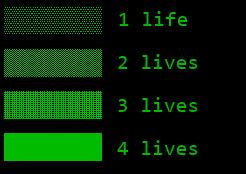
\includegraphics[scale=0.5]{figs/brikker.png}
\caption{Sådan ser brikkerne ud.}
\label{fig:brik}
\end{figure}
		

\section{Display}
\begin{itemize}
\item Videobuffer
\item Opdatere LED i interrupt
\end{itemize}

\section{Styring med rat}
\begin{itemize}
\item Gameport breakout board
\item Gameport driver
\item ADC-converter
\item (Kalibreringsrutine og linearitet)
\item Manuel kalibrering
\end{itemize}


\section{Rettelser og fintuning}
\begin{itemize}
\item Random vinkel den bliver roteret hver gang den reflekteres for at bolden ikke bliver fanget i mønstre
\item Justeret hastighed og lavet så den kun tegner bolden hver anden gang
\end{itemize}